\documentclass[9pt,landscape]{article}
\usepackage{multicol}
\usepackage{calc}
\usepackage{ifthen}
\usepackage[landscape]{geometry}
\usepackage{amsmath,amsthm,amsfonts,amssymb}
\usepackage{color,graphicx,overpic}
\usepackage[bookmarks=false]{hyperref}
\usepackage{wrapfig}
\usepackage{eso-pic}
\usepackage[defaultfam,tabular,lining]{montserrat} 
\usepackage{float}
\usepackage{tabularx}
%\usepackage[dvipsnames, table]{xcolor}
\usepackage{blindtext}\documentclass[9pt,landscape]{article}
\usepackage{multicol}
\usepackage{calc}
\usepackage{ifthen}
\usepackage[landscape]{geometry}
\usepackage{amsmath,amsthm,amsfonts,amssymb}
\usepackage{color,graphicx,overpic}
\usepackage[bookmarks=false]{hyperref}
\usepackage{wrapfig}
\usepackage{eso-pic}
\usepackage[defaultfam,tabular,lining]{montserrat} 
\usepackage{float}
\usepackage{tabularx}
%\usepackage[dvipsnames, table]{xcolor}
\usepackage{blindtext}
\usepackage{multirow}
\usepackage{listings}
\usepackage[x11names]{xcolor}
%\usepackage[dvipsnames]{xcolor}
\ProvidesPackage{pythonhighlight}[2011/09/19 python code highlighting; provided by Olivier Verdier <olivier.verdier@gmail.com>]
%Path relative to the main .tex file
\graphicspath{ {./static/} }

\pdfinfo{
  /Title (PyAnsys Cheatsheets)
  /Creator (TeX)
  /Producer (pdfTeX 1.40.0)
  /Author (Ansys Inc.,)
  /Subject (PyMAPDL)
  /Keywords (PyMAPDL,MAPDL,ANSYS,FEA)}

% This sets page margins to .5 inch if using letter paper, and to 1cm
% if using A4 paper. (This probably isn't strictly necessary.)
% If using another size paper, use default 1cm margins.
\ifthenelse{\lengthtest { \paperwidth = 11in}}
    { \geometry{top=.15in,left=.25in,right=.25in,bottom=.1in} }
    {\ifthenelse{ \lengthtest{ \paperwidth = 297mm}}
        {\geometry{top=1cm,left=1cm,right=1cm,bottom=1cm} }
        {\geometry{top=1cm,left=1cm,right=1cm,bottom=1cm} }
    }

% Turn off header and footer
\pagestyle{empty}

% Redefine section commands to use less space
\makeatletter
\renewcommand{\section}{\@startsection{section}{1}{0mm}%
                                {-1ex plus -.5ex minus -.2ex}%
                                {0.5ex plus .2ex}%x
                                {\normalfont\large\bfseries}}
\renewcommand{\subsection}{\@startsection{subsection}{2}{0mm}%
                                {-1explus -.5ex minus -.2ex}%
                                {0.5ex plus .2ex}%
                                {\normalfont\normalsize\bfseries}}
\renewcommand{\subsubsection}{\@startsection{subsubsection}{3}{0mm}%
                                {-1ex plus -.5ex minus -.2ex}%
                                {1ex plus .2ex}%
                                {\normalfont\small\bfseries}}
\makeatother

\definecolor{silver}{RGB}{217,216,214}
\definecolor{gold}{RGB}{255,183,27}
\definecolor{steel}{RGB}{137,138,141}
\definecolor{lead}{RGB}{55,58,54}
\definecolor{bronze}{RGB}{200,146,17}
\definecolor{cblack}{RGB}{0,0,0}
\definecolor{codegreen}{rgb}{0,0.6,0}
\definecolor{codegray}{rgb}{0.5,0.5,0.5}
\definecolor{codepurple}{rgb}{0.58,0,0.82}

\lstdefinestyle{python_style}{
	backgroundcolor=\color{white},
	%commentstyle=\color{white},
	%keywordstyle=\color{gold},
	%stringstyle=\color{cblack}
	%backgroundcolor=\color{backcolour},   
	commentstyle=\color{codegreen},
	keywordstyle=\color{magenta},
	numberstyle=\tiny\color{codegray},
	stringstyle=\color{codepurple},
	frame=single,
	breaklines,
	%basicstyle=\sffamily\footnotesize,
	basicstyle=\ttfamily,
	showspaces=false,
	showstringspaces=false,
    	showtabs=false,
	%tabsize=2
}

\lstset{style=python_style}

\def\code#1{\texttt{#1}}

% Define BibTeX command
\def\BibTeX{{\rm B\kern-.05em{\sc i\kern-.025em b}\kern-.08em
    T\kern-.1667em\lower.7ex\hbox{E}\kern-.125emX}}

% Don't print section numbers
\setcounter{secnumdepth}{0}


\setlength{\parindent}{0pt}
\setlength{\parskip}{0pt plus 0.5ex}

%My Environments
\newtheorem{example}[section]{Example}
% -----------------------------------------------------------------------

\begin{document}
\raggedright
\footnotesize
\begin{center}
     \Huge{\textbf{Cheatsheet for PyMAPDL}} \\
\end{center}
\AddToShipoutPicture*
	{\put(670,577.5){
\includegraphics[height = 1.2cm]{ansys.png}}}
\AddToShipoutPictureBG*{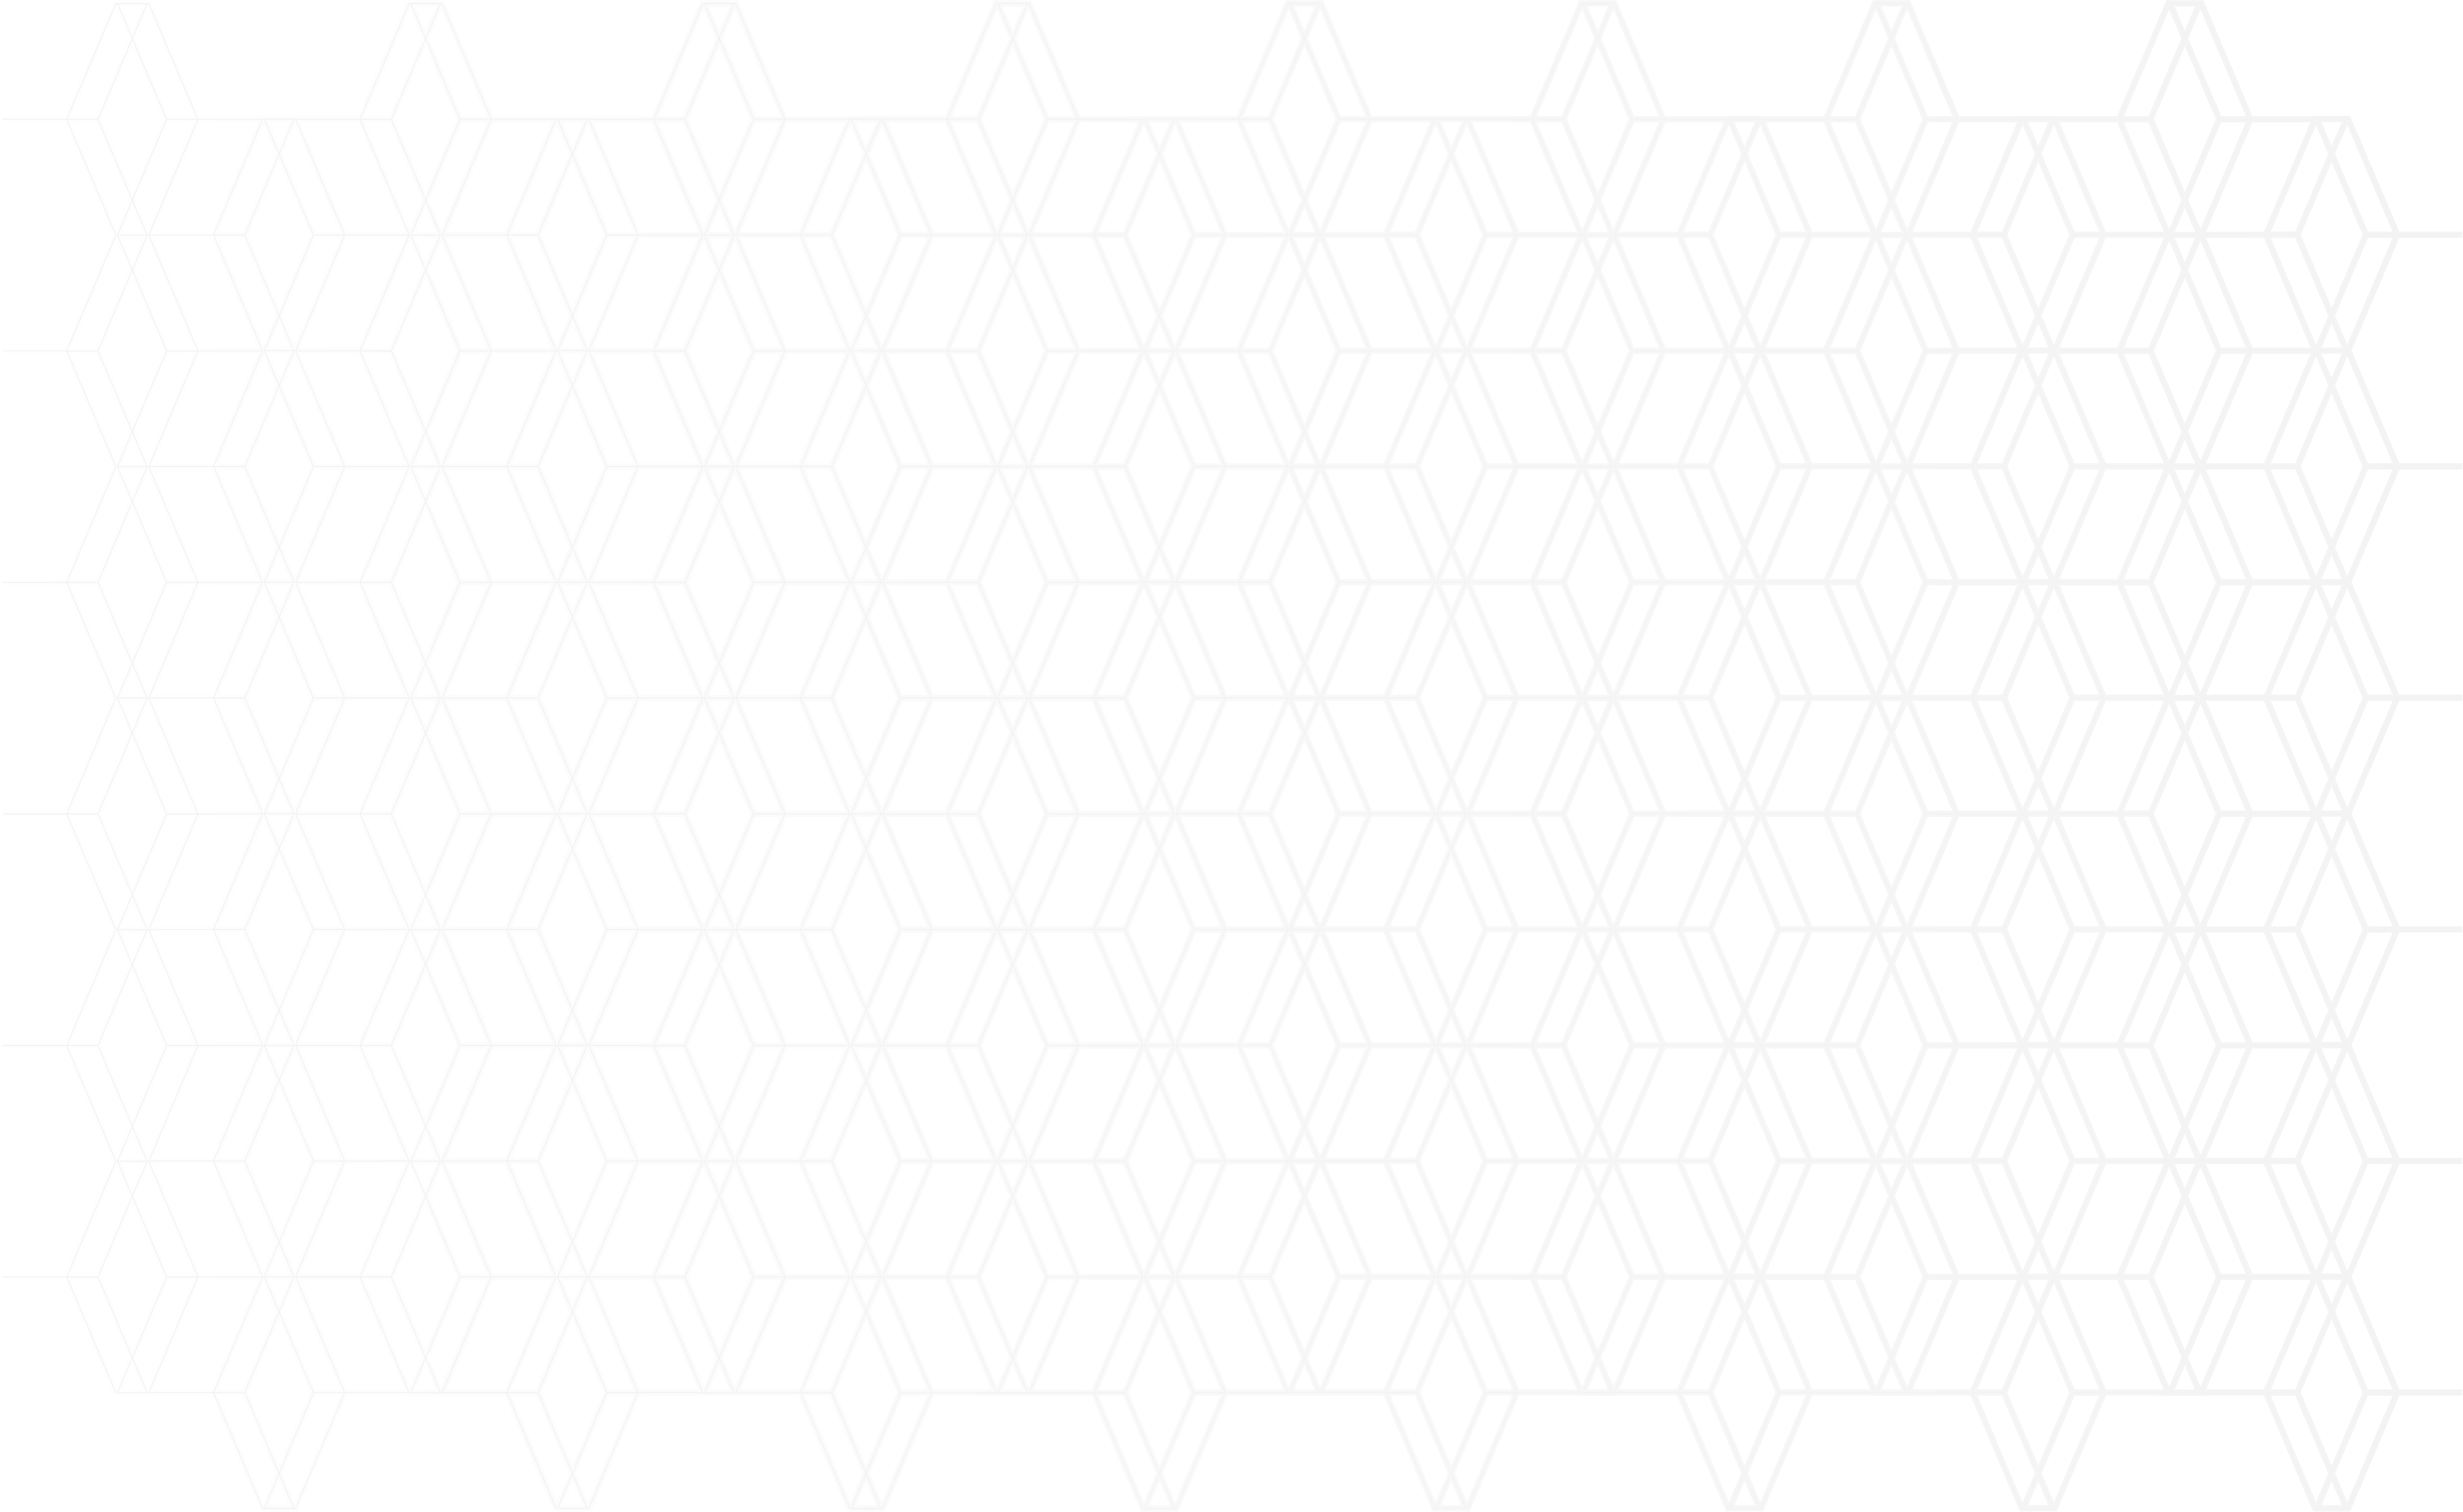
\includegraphics[width=\paperwidth]{bground_2.png}}
\vspace{-0.15cm}
\noindent\makebox[\linewidth]{\rule{\paperwidth}{2pt}}

\begin{multicols}{3}
% multicol parameters
% These lengths are set only within the two main columns
%\setlength{\columnseprule}{0.25pt}
\setlength{\premulticols}{1pt}
\setlength{\postmulticols}{1pt}
\setlength{\multicolsep}{1pt}
\setlength{\columnsep}{2pt}

\section{
\includegraphics[height=\fontcharht\font`\S]{slash.png} Launching PyMAPDL}
To launch PyMAPDL instance locally and exit it
\begin{lstlisting}[language=Python]
# To launch an instance
from ansys.mapdl.core import launch_mapdl
mapdl=launch_mapdl()
# To exit the instance
mapdl.exit()
\end{lstlisting}

To specify a jobname, number of processors, and working directory
\begin{lstlisting}[language=Python]
jname='user_jobname'
path='<path of directory>'
mapdl=launch_mapdl(nproc=2,run_location=path,
                   jobname=jname)
\end{lstlisting}

To connect to an existing instance of MAPDL at IP 192.168.1.30 and port 50001.
\begin{lstlisting}[language=Python]
mapdl=launch_mapdl
            (start_instance=False,
             ip='192.168.1.30',port=50001)
\end{lstlisting}
To create and exit a pool of instances
\begin{lstlisting}[language=Python]
# To create a pool of 10 instances
from ansys.mapdl.core import LocalMapdlPool
pool=mapdl.LocalMapdlPool(10)
# To exit the pool
pool.exit()
\end{lstlisting}

\section{
\includegraphics[height=\fontcharht\font`\S]{slash.png} PyMAPDL Language}
PyMAPDL commands are Python statements that act as a wrapper for APDL commands. For instance, \code{ESEL,s,type,,1} is translated as
\begin{lstlisting}[language=Python]
mapdl.esel('s','type',vmin=1) 
\end{lstlisting}

Commands that start with * or / have those characters removed.
\begin{lstlisting}[language=Python]
mapdl.prep7()	# /PREP7
mapdl.get()	# *GET
\end{lstlisting}

In cases where removing * or / will cause conflict with other commands, a prefix "slash" or "star" is added.
\begin{lstlisting}[language=Python]
mapdl.solu()		# SOLU
mapdl.slashsolu()	# /SOLU

mapdl.vget()		# VGET
mapdl.starvget()	# *VGET
\end{lstlisting} 

\columnbreak
Converting an existing APDL script to PyMAPDL format
\begin{lstlisting}[language=Python]
inputfile='ansys_inputfile.inp'
pyscript='pyscript.py'
mapdl.convert_script(inputfile,pyscript)
\end{lstlisting} 

\section{
\includegraphics[height=\fontcharht\font`\S]{slash.png} MAPDL Class}
Load a table from Python to MAPDL
\begin{lstlisting}[language=Python]
mapdl.load_table(name,array,var1='',var2='',
                 var3='',csysid='')
\end{lstlisting} 

To access from or write parameters to MAPDL database
\begin{lstlisting}[language=Python]
# Save a parameter to a NumPy array nparray
nparray=mapdl.parameters['displ_load']
# Create a parameterfrom a NumPy array nparray
mapdl.parameters['exp_disp']=nparray
\end{lstlisting} 

To access information using \code{*GET} and \code{*VGET} directly to NumPy arrays
\begin{lstlisting}[language=Python]
# Runs *GET command and returns a Python value
mapdl.get_value(entity='',entnum='',
                item1='',it1num='',
                item2='',it2num='',**kwargs)

# Runs *VGET command and returns a Python array
mapdl.get_array(entity='',entnum='',
                item1='', it1num='', item2='',
                it2num='',kloop='',**kwargs)
\end{lstlisting} 
\vfill

\section{
\includegraphics[height=\fontcharht\font`\S]{slash.png} Mesh Class}
Store the finite element mesh as a VTK UnstructuredGrid data object.
\begin{lstlisting}[language=Python]
grid=mapdl.mesh.grid
\end{lstlisting} 

Save element \& node numbers to Python arrays.
\begin{lstlisting}[language=Python]
# Array of nodal coordinates
nodes=mapdl.mesh.nodes

# Save node numbers of selected nodes to array
node_num=mapdl.mesh.nnum
# Save node numbers of all nodes to array
node_num_all=mapdl.mesh.nnum_all

# Element numbs. of currently selected elements
elem_num=mapdl.mesh.enum
# All element numbers incl. those not selected
elem_num_all=mapdl.mesh.enum_all
\end{lstlisting} 
\vfill

\columnbreak

\section{
\includegraphics[height=\fontcharht\font`\S]{slash.png} Post-processing Class}
%To plot results the general form is: \code{mapdl.postprocessing.result_name}
This class is used for plotting and saving results to NumPy arrays.
\begin{lstlisting}[language=Python]
mapdl.post1()
mapdl.set(1, 2)
# Plot the nodal equivalent stress
mapdl.post_processing.plot_nodal_eqv_stress()
# Save nodal eqv. stresses to a Python array
nod_eqv_stress=
       mapdl.post_processing.nodal_eqv_stress()
# Plot contour legend using dictionary
mapdl.allsel()
sbar_kwargs={"color": "black",
          "title": "Equivalent Stress (psi)",
        "vertical": False,"n_labels": 6}
mapdl.post_processing.plot_nodal_eqv_stress(
                  cpos='xy',
                  background='white',
                  edge_color='black',
                  show_edges=True,
                  scalar bar_args=sbar_kwargs,
                  n_colors=9)
\end{lstlisting} 
\vfill
\section{
\includegraphics[height=\fontcharht\font`\S]{slash.png} Plotting Class}
Plotting is interpolated with pyvista by saving the resulting stress and storing wtihin the underlying UnstructuredGrid
\begin{lstlisting}[language=Python]
pl=pyvista.Plotter()
pl0=mapdl.post_processing.plot_nodal_stress(
      return_plotter=True)
pl.add(pl0.mesh)
pl.show()
\end{lstlisting} 
\begin{lstlisting}[language=Python]
# Plot the currently selected elements
mapdl.eplot(show_node_numbering, vtk)
# Plot the selected volumes
mapdl.vplot(nv1, nv2, ninc, degen, scale, ...)
# Display the selected areas
mapdl.aplot(na1, na2, ninc, degen, scale, ...)
# Display the selected lines without 
# MAPDL plot symbols
mapdl.lplot(vtk=True, cpos='xy', line_width=10)
# Save png file of line plot with MAPDL 
# coordinate symbol
mapdl.psymb('CS', 1)
mapdl.lplot(vtk=False)
\end{lstlisting} 
\vfill

\subsection{References from PyMAPDL Documentation}
\begin{itemize}
\item \href{https://mapdldocs.pyansys.com/getting_started/index.html}{Getting Started}
\item \href{https://mapdldocs.pyansys.com/mapdl_commands/index.html}{MAPDL Commands}
\item \href{https://mapdldocs.pyansys.com/api/index.html}{API Reference}
\end{itemize}
\end{multicols}
\vspace{-0.15cm}
\noindent\makebox[\linewidth]{\rule{\paperwidth}{4pt}}
\begin{center}
Getting Started With PyMAPDL 
\includegraphics[height=\fontcharht\font`\S]{slash.png} \href{https://github.com/pyansys/pymapdl}{PyMAPDL on GitHub} 
\includegraphics[height=\fontcharht\font`\S]{slash.png} Visit \code{\href{https://mapdldocs.pyansys.com/}{mapdldocs.pyansys.com}}
\end{center}
\end{document}
\usepackage{multirow}
\usepackage{listings}
\usepackage[x11names]{xcolor}
%\usepackage[dvipsnames]{xcolor}

\pdfinfo{
  /Title (example.pdf)
  /Creator (TeX)
  /Producer (pdfTeX 1.40.0)
  /Author (Seamus)
  /Subject (Example)
  /Keywords (pdflatex, latex,pdftex,tex)}

% This sets page margins to .5 inch if using letter paper, and to 1cm
% if using A4 paper. (This probably isn't strictly necessary.)
% If using another size paper, use default 1cm margins.
\ifthenelse{\lengthtest { \paperwidth = 11in}}
    { \geometry{top=.25in,left=.35in,right=.35in,bottom=.1in} }
    {\ifthenelse{ \lengthtest{ \paperwidth = 297mm}}
        {\geometry{top=1cm,left=1cm,right=1cm,bottom=1cm} }
        {\geometry{top=1cm,left=1cm,right=1cm,bottom=1cm} }
    }

% Turn off header and footer
\pagestyle{empty}

% Redefine section commands to use less space
\makeatletter
\renewcommand{\section}{\@startsection{section}{1}{0mm}%
                                {-1ex plus -.5ex minus -.2ex}%
                                {0.5ex plus .2ex}%x
                                {\normalfont\large\bfseries}}
\renewcommand{\subsection}{\@startsection{subsection}{2}{0mm}%
                                {-1explus -.5ex minus -.2ex}%
                                {0.5ex plus .2ex}%
                                {\normalfont\normalsize\bfseries}}
\renewcommand{\subsubsection}{\@startsection{subsubsection}{3}{0mm}%
                                {-1ex plus -.5ex minus -.2ex}%
                                {1ex plus .2ex}%
                                {\normalfont\small\bfseries}}
\makeatother

\definecolor{silver}{RGB}{217,216,214}
\definecolor{gold}{RGB}{255,183,27}
\definecolor{steel}{RGB}{137,138,141}
\definecolor{lead}{RGB}{55,58,54}
\definecolor{bronze}{RGB}{200,146,17}
\definecolor{cblack}{RGB}{0,0,0}

\lstdefinestyle{python_style}{
	backgroundcolor=\color{silver},
	commentstyle=\color{DarkGoldenrod3},
	keywordstyle=\color{cblack},
	frame=single,
	breaklines,
	basicstyle=\sffamily\footnotesize,
	%basicstyle=\ttfamily\small,
	showspaces=false
	showstringspaces=false,
    	showtabs=false,
	%tabsize=2
	stringstyle=\color{lead}
}

\lstset{style=python_style}

\def\code#1{\texttt{#1}}

% Define BibTeX command
\def\BibTeX{{\rm B\kern-.05em{\sc i\kern-.025em b}\kern-.08em
    T\kern-.1667em\lower.7ex\hbox{E}\kern-.125emX}}

% Don't print section numbers
\setcounter{secnumdepth}{0}


\setlength{\parindent}{0pt}
\setlength{\parskip}{0pt plus 0.5ex}

%My Environments
\newtheorem{example}[section]{Example}
% -----------------------------------------------------------------------

\begin{document}
\raggedright
\footnotesize
\begin{center}
     \Huge{\textbf{Cheatsheet for PyMAPDL}} \\
\end{center}

\AddToShipoutPicture*
	{\put(670,560){
\includegraphics[height = 1.25cm]{ansys.png}}}

\AddToShipoutPictureBG*{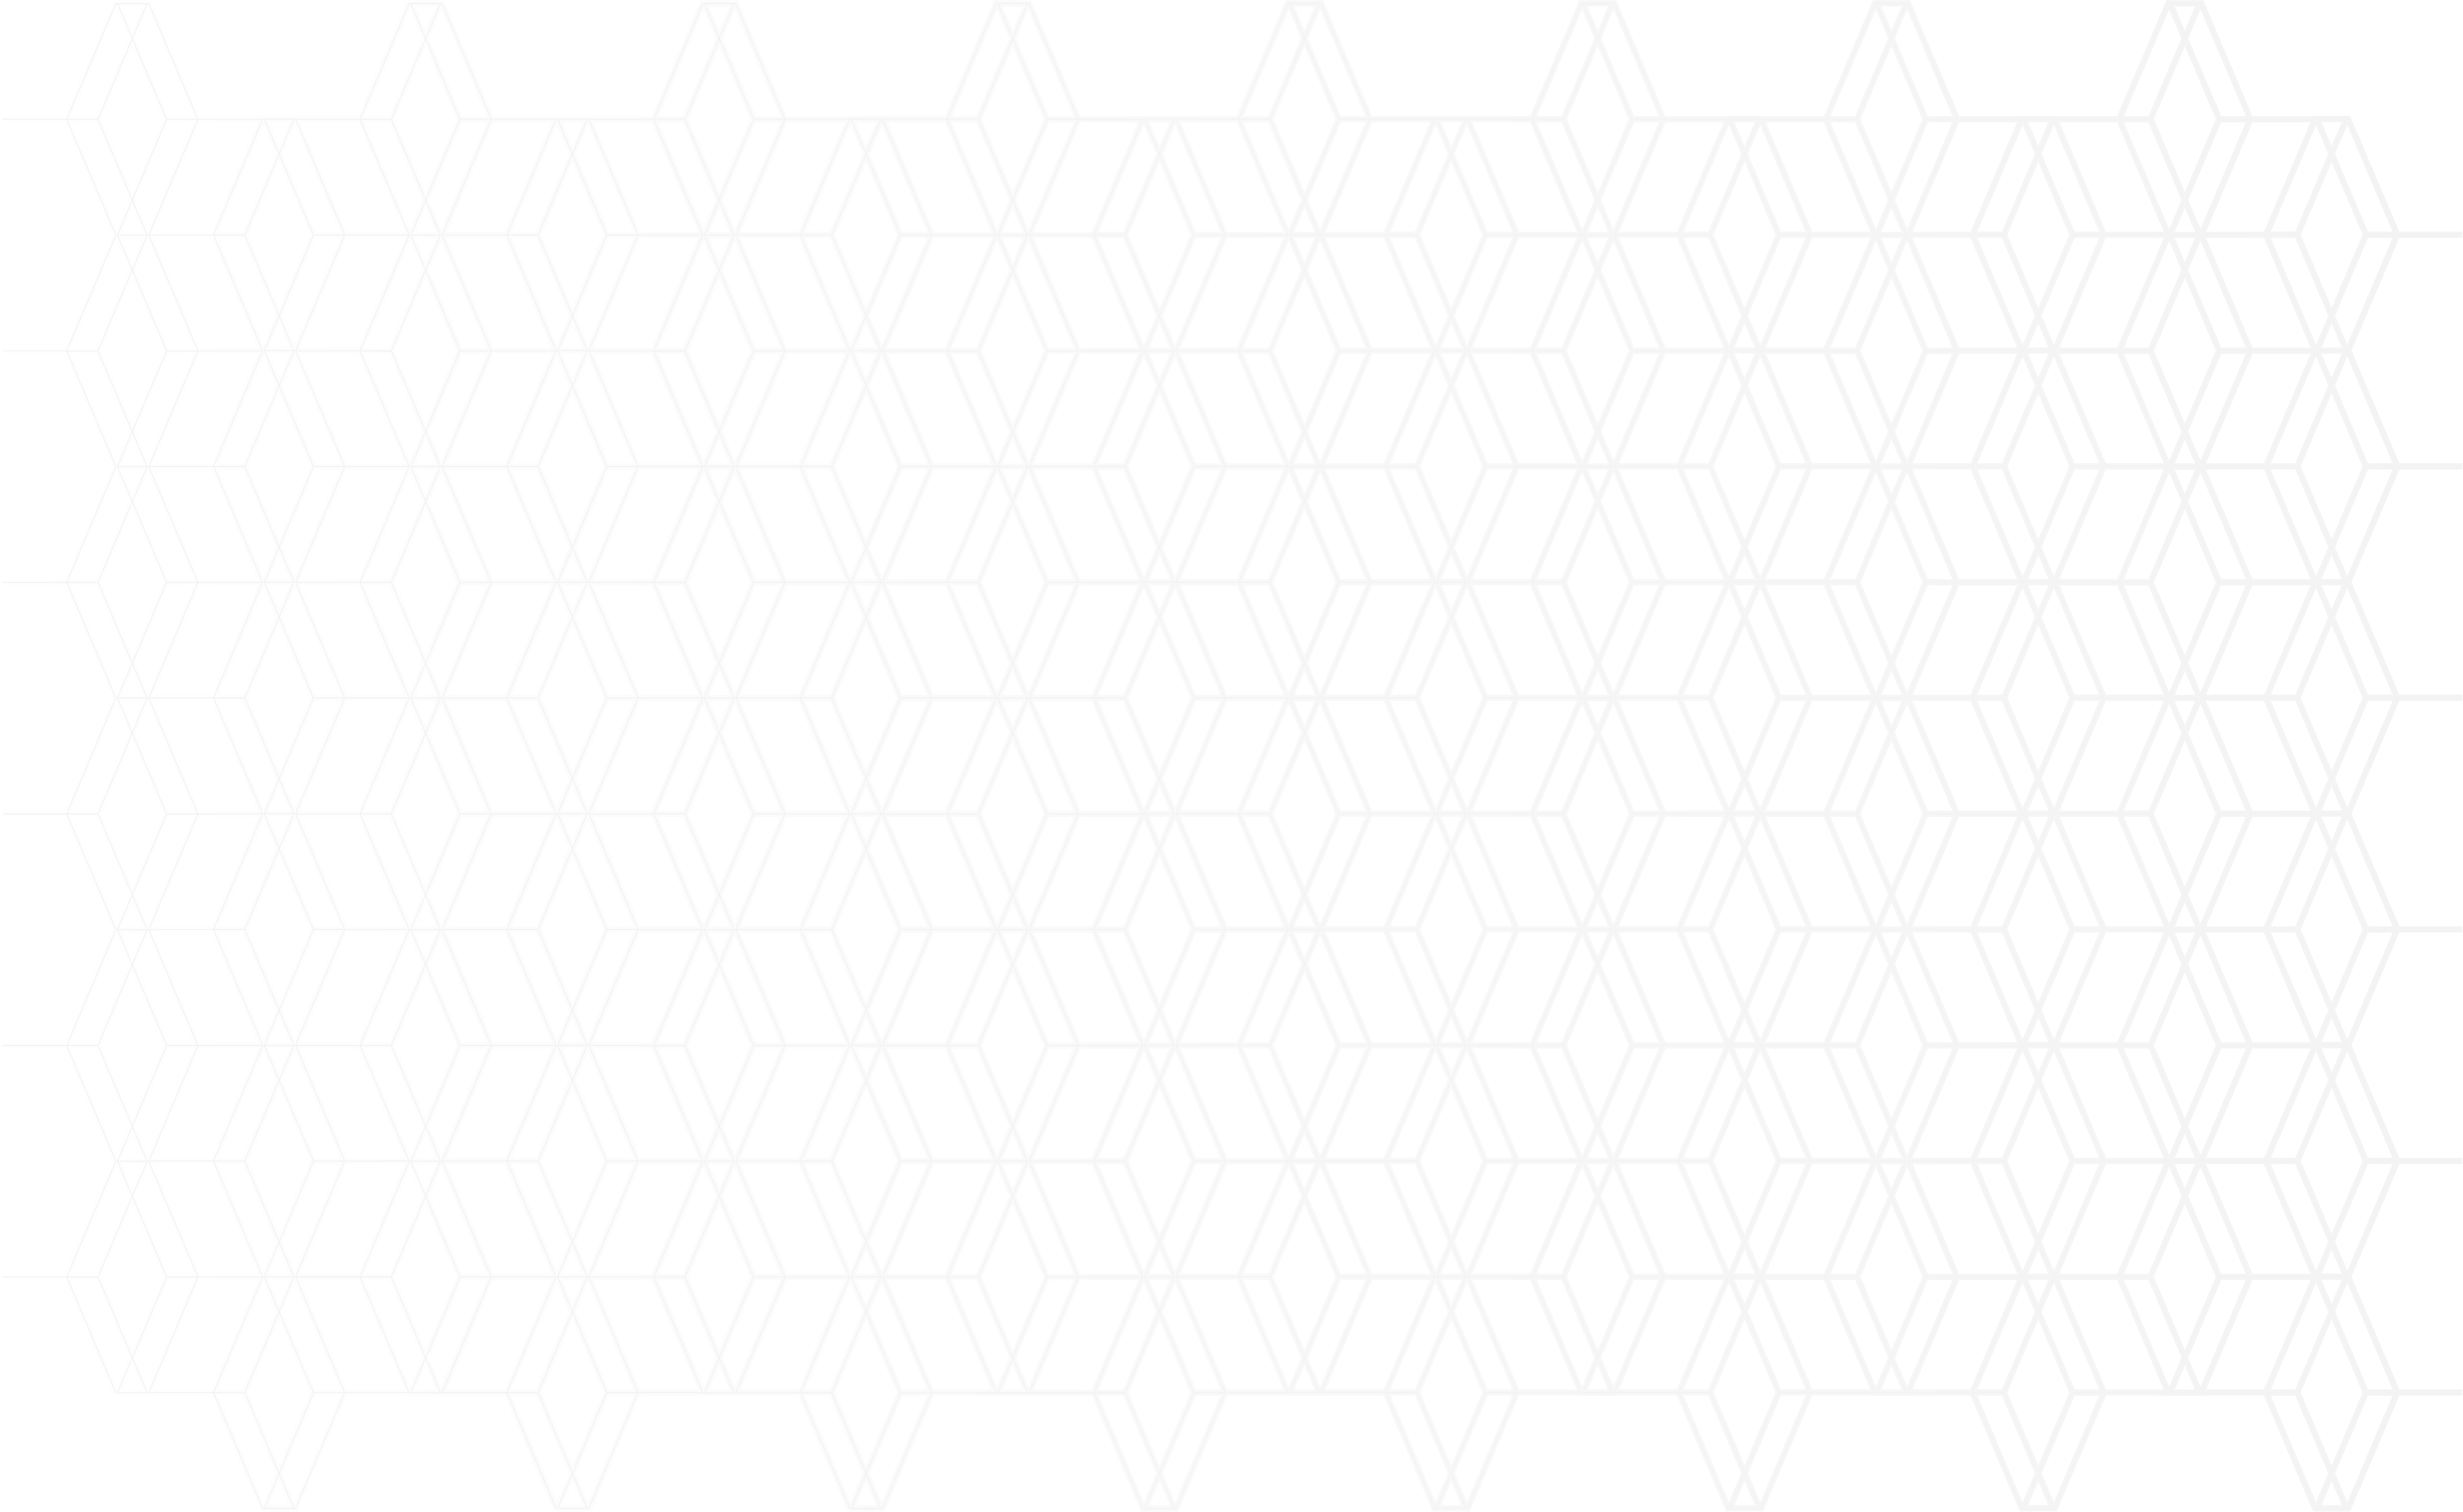
\includegraphics[width=\paperwidth]{bground_2.png}}

\noindent\makebox[\linewidth]{\rule{\paperwidth}{2pt}}

\begin{multicols}{3}
% multicol parameters
% These lengths are set only within the two main columns
%\setlength{\columnseprule}{0.25pt}
\setlength{\premulticols}{1pt}
\setlength{\postmulticols}{1pt}
\setlength{\multicolsep}{1pt}
\setlength{\columnsep}{2pt}

\section{
\includegraphics[height=\fontcharht\font`\S]{slash.png} Launching PyMAPDL}
To launch PyMAPDL instance locally and exit it
\begin{lstlisting}[language=Python]
# To launch an instance
from ansys.mapdl.core import launch_mapdl
mapdl=launch_mapdl()
# To exit the instance
mapdl.exit()
\end{lstlisting}

To specify a jobname, number of processors, and working directory
\begin{lstlisting}[language=TeX]
jname='user_jobname'
path = <path of directory>
mapdl=launch_mapdl(nproc=2,run_location=path,jobname=jname)
\end{lstlisting}

To create and exit a pool of instances
\begin{lstlisting}[language=Python]
# To create a pool of 10 instances
from ansys.mapdl.core import LocalMapdlPool
pool=mapdl.LocalMapdlPool(10)
# To exit the pool
pool.exit()
\end{lstlisting}

\section{
\includegraphics[height=\fontcharht\font`\S]{slash.png} PyMAPDL Language}
PyMAPDL commands are Python statements that act as a wrapper for APDL commands. For instance, \code{ESEL,s,type,,1} is translated as
\begin{lstlisting}[language=Matlab]
mapdl.esel('s','type',vmin=1) 
\end{lstlisting}

Commands that start with * or / have those characters removed.
\begin{lstlisting}[language=Python]
mapdl.prep7()	# /PREP7
mapdl.get()	# *GET
\end{lstlisting}

In cases where removing * or / will cause conflict with other commands, a prefix "slash" or "star" is added.
\begin{lstlisting}[language=Python]
mapdl.solu()		# SOLU
mapdl.slashsolu()	# /SOLU

mapdl.vget()		# VGET
mapdl.starvget()	# *VGET
\end{lstlisting} 

Converting an existing APDL script to PyMAPDL format
\begin{lstlisting}[language=Python]
inputfile='ansys_inputfile.inp'
pyscript='pyscript.py'
mapdl.convert_script(inputfile,pyscript)
\end{lstlisting}
\columnbreak

\section{
\includegraphics[height=\fontcharht\font`\S]{slash.png} MAPDL Class}
Load a table from Python to MAPDL
\begin{lstlisting}[language=Octave]
mapdl.load_table(name,array,var1='', var2='',var3='', csysid='')
\end{lstlisting}
To access from or write parameters to MAPDL database
\begin{lstlisting}[language=Python]
# To save a parameter named 'displ_load' to a NumPy array nparray
nparray=mapdl.parameters['displ_load']
# To create a parameter named 'exp_disp' from a NumPy array nparray
mapdl.parameters['exp_disp']=nparray
\end{lstlisting}

To access information using \code{*GET} and \code{*VGET} directly to NumPy arrays
\begin{lstlisting}[language=Python]
# Runs the *GET command and returns a Python value.
mapdl.get_value(entity='', entnum='', item1='', it1num='', item2='', it2num='', **kwargs)

# Runs *VGET command and returns a Python array.
mapdl.get_array(entity='', entnum='', item1='', it1num='', item2='', it2num='', kloop='', **kwargs)
\end{lstlisting}
\vfill

\section{
\includegraphics[height=\fontcharht\font`\S]{slash.png} Mesh Class}
Store the finite element mesh as a VTK UnstructuredGrid data object.
\begin{lstlisting}[language=Python]
grid = mapdl.mesh.grid
\end{lstlisting}

Save element \& node numbers to Python arrays.
\begin{lstlisting}[language=Python]
# Array of nodal coordinates
nodes=mapdl.mesh.nodes

# Save node numbers of selected nodes to array
node_num=mapdl.mesh.nnum
# Save node numbers of selected nodes to array
node_num_all=mapdl.mesh.nnum_all

# Element numbers of currently selected elements
elem_num=mapdl.mesh.enum
# Array of all element numbers, even those not selected.
elem_num_all=mapdl.mesh.enum_all
\end{lstlisting}
\vfill

\columnbreak

\section{
\includegraphics[height=\fontcharht\font`\S]{slash.png} Post-processing Class}
To plot results the general form is: \code{mapdl.postprocessing.result\_name}

\begin{lstlisting}[language=Python]
mapdl.post1()
mapdl.set(1, 2)
# To plot the nodal equivalent stress
mapdl.post_processing.plot_nodal_eqv_stress()
# To save nodal eqv. stresses to a Python array
nod_eqv_stress=mapdl.post_processing.nodal_eqv_stress()
# To plot the contour legend or Scalar bar using python data structure dictionary
mapdl.allsel()
sbar_kwargs = {"color": "black", "title": "1st Principal Stress (psi)", "vertical": False, "n_labels": 6}
mapdl.post_processing.plot_nodal_principal_stress('1', cpos='xy', background='white', edge_color='black', show_edges=True, scalar bar_args=sbar_kwargs, n_colors=9)
\end{lstlisting}
\vfill
\section{
\includegraphics[height=\fontcharht\font`\S]{slash.png} Plotting Class}
Plotting is interpolated with pyvista by saving the resulting stress and storing wtihin the underlying UnstructuredGrid
\begin{lstlisting}[language=Python]
pl = pyvista.Plotter()
pl0 = mapdl.post_processing.plot_nodal_stress(return_plotter=True)
pl.add(pl0.mesh)
pl.show()
\end{lstlisting}
\begin{lstlisting}[language=Python]
# To plot the currently selected elements
mapdl.eplot(show_node_numbering, vtk)
# To plot the selected volumes
mapdl.vplot(nv1, nv2, ninc, degen, scale, ...)
# To display the selected areas
mapdl.aplot(na1, na2, ninc, degen, scale, ...)
# To display the selected lines without MAPDL plot symbols
mapdl.lplot(vtk=True, cpos='xy', line_width=10)
# To save a '.png' file of the line plot with MAPDL coordinate symbol
mapdl.psymb('CS', 1)
mapdl.lplot(vtk=False)
\end{lstlisting}
\vfill
%\section{
\includegraphics[height=\fontcharht\font`\S]{slash.png} MAPDL Math Class}
%\begin{lstlisting}[language=Python]
%# To add two APDL Math vectors or matrices
%math.MapdlMath.add(obj1, obj2)
%# To solve an eigenproblem
%math.MapdlMath.eigs(nev, k[, m, c, phi, algo, ...]) 
%# To send a scipy matrix or numpy array to MAPDL
%math.MapdlMath.matrix(matrix[, name, triu])
%# To perform the matrix operation:M2= v*M1 + w*M2
%math.ApdlMathObj.axpy(op, val1, val2) 
%# To return if matrix is symmetric
%math.Ansmat.sym()
%# To solve a linear system
%math.AnsSolver.solve(b[,x])
%\end{lstlisting}
%\vfill
\subsection{References from PyMAPDL Documentation}
\begin{itemize}
\item \href{https://mapdldocs.pyansys.com/getting_started/index.html}{Getting Started}
\item \href{https://mapdldocs.pyansys.com/mapdl_commands/index.html}{MAPDL Commands}
\item \href{https://mapdldocs.pyansys.com/api/index.html}{API Reference}
\end{itemize}

\end{multicols}
\vfill
\noindent\makebox[\linewidth]{\rule{\paperwidth}{4pt}}
\begin{center}
Getting Started With PyMAPDL 
\includegraphics[height=\fontcharht\font`\S]{slash.png} Ansys Innovation Courses 
\includegraphics[height=\fontcharht\font`\S]{slash.png} Visit \code{\href{https://courses.ansys.com/}{ansys.com/courses}}
\end{center}
\end{document}